\begin{enumerate}[label=\thesection.\arabic*.,ref=\thesection.\theenumi]
\numberwithin{equation}{enumi}

\item For a unity feedback system shown in \ref{fig:ee18btech11044_1}, $\frac{10}{s(s+1)}$. Design a lead compensator such that the phase margin of the system is 45$^{\circ}$ and appropriate steady state error is less than or equal to $\frac{1}{15}$ units of the final output value. Further the gain crossover frequency of the system must be less than 7.5rad/sec. \\


\item For the control system shown in \ref{fig:ee18btech11044_1} write the steady state output for step input. \\
\solution
\begin{align}
\lim_{t\to\infty} y(t)  = \lim_{s\to0} sY(s) \\
\lim_{s\to0} sY(s) = \lim_{s\to0}  \frac{s R(s) G(s)}{1+G(s)} \\
\lim_{s\to0} sY(s) = \lim_{s\to0} \frac{G(s)}{1 + G(s)}
\end{align}
\begin{figure}[!ht]
	\begin{center}
		\resizebox{\columnwidth}{!}{\tikzstyle{block} = [draw, fill=white, rectangle, 
    minimum height=1cm, minimum width=1cm]
\tikzstyle{sum} = [draw, fill=white, circle, node distance=1cm]
\tikzstyle{input} = [coordinate]
\tikzstyle{output} = [coordinate]
\tikzstyle{pinstyle} = [pin edge={to-,thin,black}]


% The block diagram code is probably more verbose than necessary
\begin{tikzpicture}[auto, node distance=2cm,>=latex']
    % We start by placing the blocks
    \node [input, name=input] {X(s)};
    \node [sum, right of=input] (sum) {};
    
    \node [block, right of=sum] (system) {$G(s)$ };
   
    % We draw an edge between the controller and system block to 
    % calculate the coordinate u. We need it to place the measurement block. 
    
    \node [output, right of=system] (output) {};
    \node [block, below of=system] (measurements) {1};

    % Once the nodes are placed, connecting them is easy. 
    \draw [draw,->] (input) -- node {$R(s)$} (sum);
    \draw [->] (sum) -- node {} (system);
    \draw [->] (system) -- node [name=y] {$Y(s)$}(output);
    \draw [->] (y) |- (measurements);
    \draw [->] (measurements) -| node[pos=0.99] {$-$} 
        node [near end] {} (sum);
\end{tikzpicture}
}
	\end{center}
\caption{}
\label{fig:ee18btech11044_1}
\end{figure}

\item What do you mean by steady state error and write the expression for steady state error for control system shown in \ref{fig:ee18btech11044_1} considering step input. \\
\solution 
Steady-state error is the difference between the input and the output for a prescribed test input as time tends to infinity.
\begin{align}
    e_{ss} = \lim_{s\to0} \frac{1}{1 +G(s)}
\end{align}


\item Write the general expression for the transfer function of a phase lead compensator. \\
\solution 
\begin{align}
    G_c(s) =  K_{comp}    \frac{(1+\alpha T s)}{(1+ T s)} 
\end{align}
\ref{fig:ee18btech11044_2} shows the compensated control system.
\begin{figure}[!ht]
	\begin{center}
		\resizebox{\columnwidth}{!}{\tikzstyle{block} = [draw, fill=white, rectangle, 
    minimum height=1cm, minimum width=1cm]
\tikzstyle{sum} = [draw, fill=white, circle, node distance=1cm]
\tikzstyle{input} = [coordinate]
\tikzstyle{output} = [coordinate]
\tikzstyle{pinstyle} = [pin edge={to-,thin,black}]


% The block diagram code is probably more verbose than necessary
\begin{tikzpicture}[auto, node distance=2cm,>=latex']
    % We start by placing the blocks
    \node [input, name=input] {X(s)};
    \node [sum, right of=input] (sum) {};
    
    \node [block, right of=sum] (system) {$G(s)$ };
    \node [block, right of=system] (comp) {$G_c(s)$ };
   
    % We draw an edge between the controller and system block to 
    % calculate the coordinate u. We need it to place the measurement block. 
    
    \node [output, right of=comp] (output) {};
    \node [block, below of=system] (measurements) {1};

    % Once the nodes are placed, connecting them is easy. 
    \draw [draw,->] (input) -- node {$R(s)$} (sum);
    \draw [->] (sum) -- node {} (system);
    \draw [->] (system) -- node {} (comp);
    \draw [->] (comp) -- node [name=y] {$Y(s)$}(output);
    \draw [->] (y) |- (measurements);
    \draw [->] (measurements) -| node[pos=0.99] {$-$} 
        node [near end] {} (sum);
\end{tikzpicture}
}
	\end{center}
\caption{}
\label{fig:ee18btech11044_2}
\end{figure}


\item Calculate the steady state output value and steady state error for the control system shown in \ref{fig:ee18btech11044_1}, where G(s) = $\frac{10}{s(s+1)}$. Consider the input to be unit step. \\
\solution \\
\textbf{Steady state value:}
\begin{align}
\lim_{t\to\infty} y(t) = \lim_{s\to0} \frac{10}{10+s(s+1)} \\
\lim_{t\to\infty} y(t) = 1
\end{align}
\textbf{Steady state error:}
\begin{align}
e_{ss} = \lim_{s\to0} \frac{s(s+1)}{10 + s(s+1)} \\
e_{ss} = 0
\end{align}

\item Choose a value of $K_{comp}$ which satisfies the steady state error condition. \\
\solution As the steady state error for unit step response is always zero, any value of $K_{comp}$ satisfies the steady state error condition in compensated system. For simplicity let us choose $K_{comp}$ = 1.

\item Calculate phase margin and gain cross over frequency of open-loop transfer function G(S). \\
\solution \\
\textbf{Gain cross over frequency}:
\begin{align}
    G(j\omega) = \frac{10}{j\omega (j\omega + 1)} \\
    |G(j\omega)| = \frac{10}{\sqrt{\omega^4 +\omega^2}} \\
    \frac{10}{\sqrt{\omega^4 +\omega^2}} = 1 \\
    \omega_{gc} = 3.084
\end{align}
\textbf{Phase Margin}:
\begin{align}
    \phi =  -90^{\circ} - tan^{-1}(\omega) \\ 
    pm = 180^{\circ} -90^{\circ} - tan^{-1}(\omega_{gc}) \\ 
    pm = 17.966^{\circ} \\ 
\end{align}
\item Write the expression for maximum phase of a lead compensator and the frequency where it occurs \\
\solution 
\begin{align}
    \phi_{max} = sin^{-1}(\frac{\alpha - 1}{\alpha + 1}) \label{eq:ee18btech11044_1} \\
    \omega_m = \frac{1}{T \alpha} \label{eq:ee18btech11044_2}
\end{align}

\item Calculate the value of $\phi_{max}$ required to meet desired phase margin. \\
\solution 
\begin{align}
    \phi_{max} = 45^{\circ} - pm + 15^{\circ} \\ 
    \phi_{max} = 45^{\circ} - 17.966^{\circ} + 15^{\circ} \\
    \phi_{max} = 42.034^{\circ}
\end{align}
Here the extra $15^o$ has been added to compensate for the shift in $\omega_{gc}$.  
\item Using \eqref{eq:ee18btech11044_1} calculate the value of $\alpha$ \\
\solution 
\begin{align}
    sin(42.034^{\circ}) = \frac{\alpha - 1}{\alpha + 1} \\
    0.669 = \frac{\alpha - 1}{\alpha + 1} \\ 
    0.331 \alpha = 1.669 \\
    \alpha = 5.04
\end{align}
\item Choose appropriate value for $\omega_m$. \\
\solution 
\begin{itemize}
    \item For maximum increase in phase margin we have to ensure that $\phi_{max}$ occurs at frequency close to $\omega_{gc}$ of G(s).
    \begin{align}
        \omega_m = 3.084 rad/sec
    \end{align}
    \item We know that $\omega_{gc}$ gets shifted slightly when we cascade a compensator to original transfer function, to compensate for the shift we have already added an extra $15^{\circ}$ to $\phi_{max}$.
\end{itemize}

\item Using \eqref{eq:ee18btech11044_2} calculate the value of T. \\
\solution
\begin{align}
    T = \frac{1}{ \omega_m \alpha} \\
    T = \frac{1}{15.54} \\
    T = 0.064
\end{align}

\item Write the final expression of the Lead compensator designed. \\
\solution
\begin{align}
    G_c(s) =   \frac{(1+ 0.322 s)}{(1+ 0.064 s)} 
\end{align}
\begin{itemize}
    \item Zero at s = -3.084
    \item Pole at s = -15.54
\end{itemize}
\item Verify using a python plot. \\
\solution
\begin{lstlisting}
codes/ee18btech11044_2.py
\end{lstlisting}

\begin{figure}[!ht]
\centering
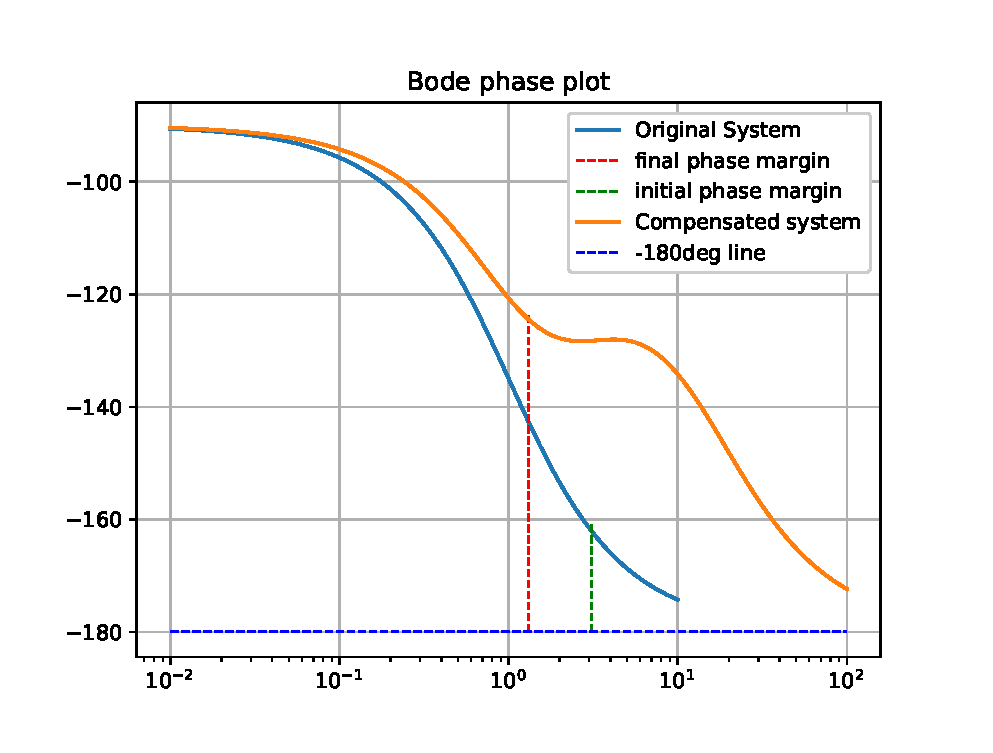
\includegraphics[width=\columnwidth]{figs/ee18btech11044_2_1.eps}
\caption{}
\end{figure}
\end{enumerate}

